\documentclass[final]{article}


\usepackage{aps360}
\makeatletter\providecommand{\@trackname}{}\makeatother
\usepackage[utf8]{inputenc}
\usepackage[T1]{fontenc}
\usepackage{hyperref}
\usepackage{url}
\usepackage{booktabs}
\usepackage{amsmath}
\usepackage{amsfonts}
\usepackage{microtype}
\usepackage{xcolor}
\usepackage{graphicx}
\usepackage{tikz}
\usetikzlibrary{arrows.meta,positioning}
\setlength{\textfloatsep}{6pt plus 1pt minus 2pt}
\setlength{\floatsep}{6pt plus 1pt minus 2pt}
\setlength{\intextsep}{6pt plus 1pt minus 2pt}
\setlength{\abovecaptionskip}{4pt}
\setlength{\belowcaptionskip}{2pt}

\title{BinSight Progress Report: Hierarchical CNN for Toronto Waste Sorting}

\author{%
  Haoyue Feng \\
  1013983076, haoyue.feng@mail.utoronto.ca\\
  GitHub: \url{https://github.com/no-where-now-here/aps360-binsight}\\
}

\begin{document}
\maketitle
\vspace{-0.55in}

\section*{Brief Project Description}
Sorting household waste in Toronto is surprisingly confusing. Residents must choose among the Blue Bin (recycling), the Green Bin (organics) and Garbage, and mistakes are common: city staff reported that about 30\% of Blue Bin material by weight is contamination~\cite{toronto2023}. Waste Wizard~\cite{wastewizard} can help, but only if the user already knows the item's name and types it in. I wanted something that works from a \emph{photo} instead.

\textbf{Input / output.} BinSight takes one RGB photo of a single household item (resized to $224\times224$) and predicts two labels: (i) the Toronto bin and (ii) the material (cardboard, paper, plastic, metal, glass, organic, other). The material head is not just ``extra information''. Many municipal exceptions---for example, a used tissue is paper but belongs in the Green Bin---show that bin is \emph{not} a simple lookup from material. The model therefore has to learn both cues together.

\textbf{Why deep learning, and what is mine?} Waste items look very different from photo to photo (crushed, dirty, shiny, dark food scraps, cluttered backgrounds). Hand-crafted features struggle with that~\cite{thung2016}, while CNNs can learn texture and shape from pixels. After proposal feedback, I made sure the \textbf{primary model is my own design}: a compact CNN trained from scratch with a hierarchical head (material $\to$ soft municipal rule prior $\to$ residual correction). Fine-tuned ResNet-18~\cite{he2016} is only a \emph{strong transfer baseline}; HOG+HSV+SVM~\cite{dalal2005} is the classical baseline. Figure~\ref{fig:arch} shows the idea in one picture.

\begin{figure}[!h]
\centering
\resizebox{0.98\linewidth}{!}{%
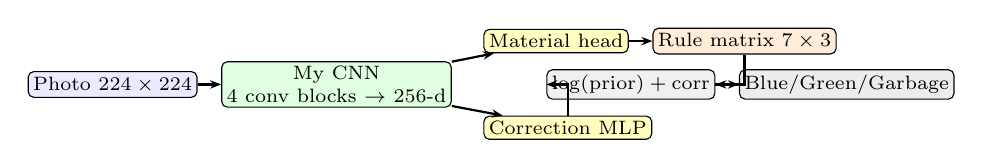
\begin{tikzpicture}[font=\scriptsize, node distance=2mm and 3mm,
  box/.style={draw, rounded corners=2pt, align=center, inner sep=1.8pt},
  arr/.style={-{Stealth[length=1.4mm]}, thick}]
  \node[box, fill=blue!8] (in) {Photo $224\times224$};
  \node[box, fill=green!12, right=of in] (cnn) {My CNN\\4 conv blocks $\to$ 256-d};
  \node[box, fill=yellow!25, above right=1mm and 4mm of cnn] (mat) {Material head};
  \node[box, fill=orange!15, right=of mat] (rule) {Rule matrix $7\times3$};
  \node[box, fill=yellow!25, below right=1mm and 4mm of cnn] (corr) {Correction MLP};
  \node[box, fill=gray!12, right=12mm of cnn] (bin) {$\log(\mathrm{prior})+\mathrm{corr}$};
  \node[box, fill=gray!15, right=of bin] (out) {Blue/Green/Garbage};
  \draw[arr] (in)--(cnn); \draw[arr] (cnn)--(mat); \draw[arr] (mat)--(rule);
  \draw[arr] (cnn)--(corr); \draw[arr] (rule)|-(bin); \draw[arr] (corr)|-(bin); \draw[arr] (bin)--(out);
\end{tikzpicture}}
\caption{Primary model in plain words: look at the photo, guess the material, turn that into a soft ``what bin does Toronto usually want?'' prior, then add a small learned correction for rule exceptions.}
\label{fig:arch}
\end{figure}

\section*{Data Processing}
Instead of inventing a brand-new camera set for this checkpoint, I \emph{repurposed and remapped} three public sources so every image has Toronto-style (material, bin) labels. That remapping is the main data contribution so far.

\textbf{Sources.} TrashNet~\cite{thung2016} (2,527 white-board studio photos), TACO~\cite{proenca2020} (I crop COCO boxes into single-object images), and the organic class of Kaggle Waste Classification~\cite{sekar2018} (needed because the other two sets have almost no Green Bin food waste).

\textbf{Cleaning steps.} (1) Crop TACO boxes with 10\% margin; drop short side $<64$\,px and \texttt{Unlabeled litter}. (2) Map every label with \texttt{data/label\_map.csv} from Waste Wizard; drop ambiguous/hazardous classes. (3) Sample 1,500 Kaggle organics and CLIP-filter drawings, posters, flowers/yard scenes (Green Bin $\neq$ yard waste). (4) pHash de-duplication (Hamming $\le4$) \emph{before} splitting. (5) Grouped stratified 70/15/15 split so all crops from one TACO photo stay together. (6) Pad to square, resize to $224\times224$, ImageNet normalisation; train-time crop/flip/rotation/colour jitter.

\begin{table}[!h]
\centering
\caption{Cleaned dataset (4419 images) after remapping and de-duplication.}
\label{tab:data}
\scriptsize
\begin{tabular}{lrrrr}
\toprule
Split & Blue & Green & Garbage & Total \\
\midrule
Train & 2108 & 762 & 227 & 3097 \\
Val / Test & 451/451 & 164/165 & 47/44 & 662/660 \\
\midrule
All & 3010 & 1091 & 318 & 4419 \\
\bottomrule
\end{tabular}
\hspace{0.3em}
\begin{tabular}{lrrr}
\toprule
Source & Blue & Green & Garbage \\
\midrule
TrashNet & 2362 & 0 & 137 \\
TACO & 648 & 13 & 181 \\
Kaggle & 0 & 1078 & 0 \\
\bottomrule
\end{tabular}
\end{table}

\begin{figure}[!h]
\centering
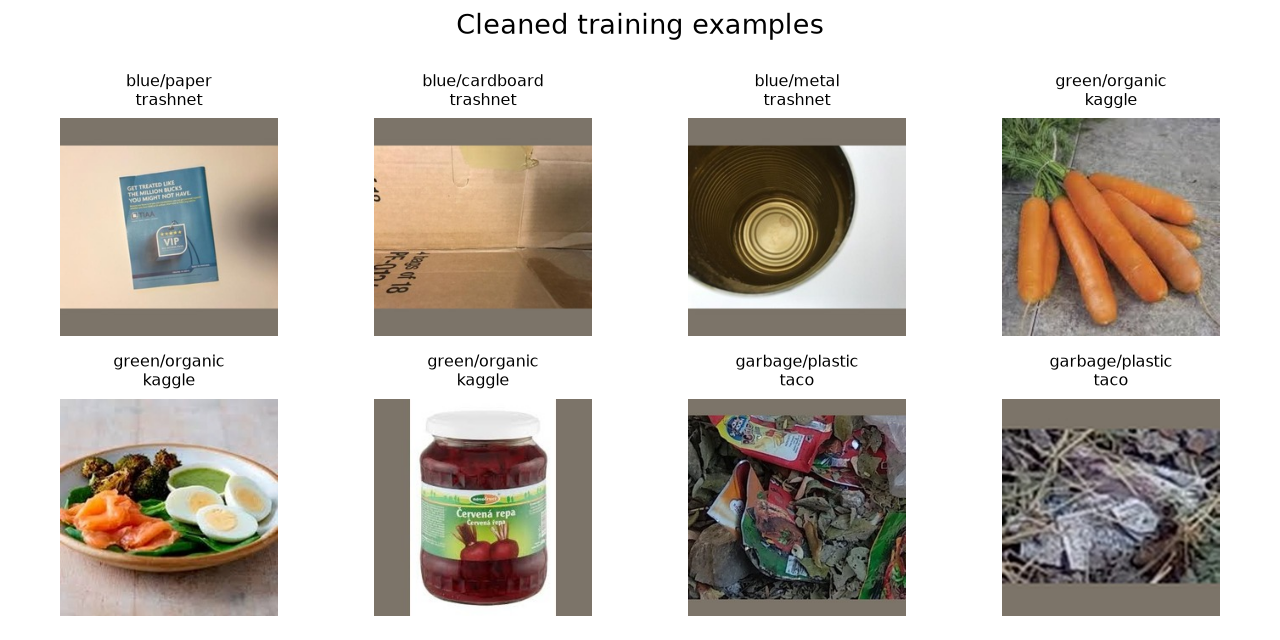
\includegraphics[height=2.55cm]{../results/data_examples.png}
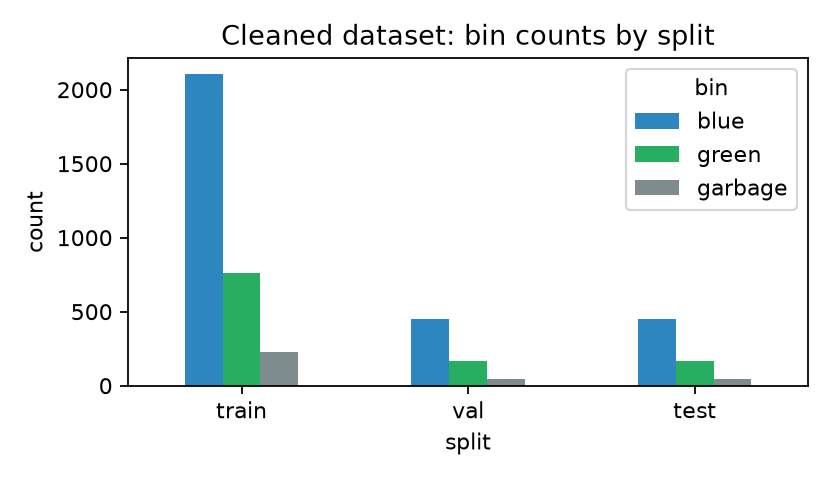
\includegraphics[height=2.55cm]{../results/data_split_bins.png}
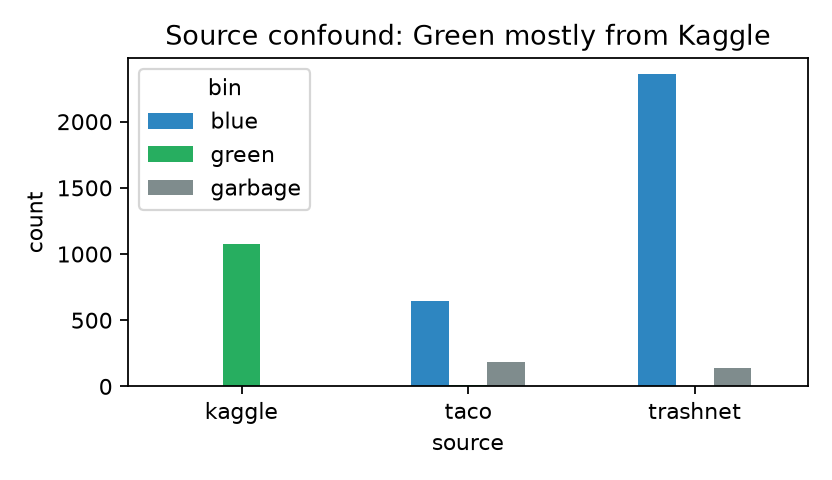
\includegraphics[height=2.55cm]{../results/data_source_bins.png}
\caption{Cleaned examples; bin counts by split (Blue dominates); source$\times$bin plot showing the Green$\approx$Kaggle \textbf{source confound}.}
\label{fig:data}
\end{figure}

\textbf{What I noticed.} The set is usable but unbalanced, and Green is almost entirely from Kaggle web images---a model could cheat by recognising photo style. Only 440/1500 TACO Flickr originals downloaded (dead links), so wild crops are fewer than planned. Even so, Table~\ref{tab:data} and Figure~\ref{fig:data} show the pipeline is finished enough to train models.

\section*{Baseline Model}
I built two baselines on the \emph{same} splits so comparisons are fair.

\textbf{Classical HOG+HSV+SVM.} If deep learning is really needed, it should beat a simple non-deep pipeline. I resize to $128\times128$, extract HOG shape features~\cite{dalal2005} (9 orientations, $16\times16$ cells, $2\times2$ blocks $\to$ 1764-d) plus an HSV histogram ($8^3=512$-d), standardise, reduce to 256-d with PCA, and train a class-balanced RBF-SVM. Validation chose $C{=}1$, $\gamma{=}10^{-3}$. This follows the spirit of TrashNet's SIFT+SVM baseline~\cite{thung2016} and is easy to reproduce in scikit-learn.

\textbf{Strong ResNet-18 baseline (not primary).} After feedback, pretrained ResNet-18 is only a transfer-learning reference~\cite{he2016}. I freeze the backbone for a few epochs, then lightly fine-tune, with the same multi-task loss $\mathrm{CE}_{\text{bin}}+\lambda\mathrm{CE}_{\text{material}}$ ($\lambda{=}0.5$) used by my primary model.

\begin{table}[!h]
\centering
\caption{Baselines on the cleaned test split.}
\label{tab:base}
\scriptsize
\begin{tabular}{lrrr}
\toprule
Model & Capacity & Test bin acc. & Macro-F1 \\
\midrule
HOG+HSV+SVM & 2276-d$\to$PCA-256 & 0.859 & 0.687 \\
ResNet-18 (freeze$\to$fine-tune) & 11.3M & 0.905 & 0.811 \\
\bottomrule
\end{tabular}
\end{table}

\begin{figure}[!h]
\centering
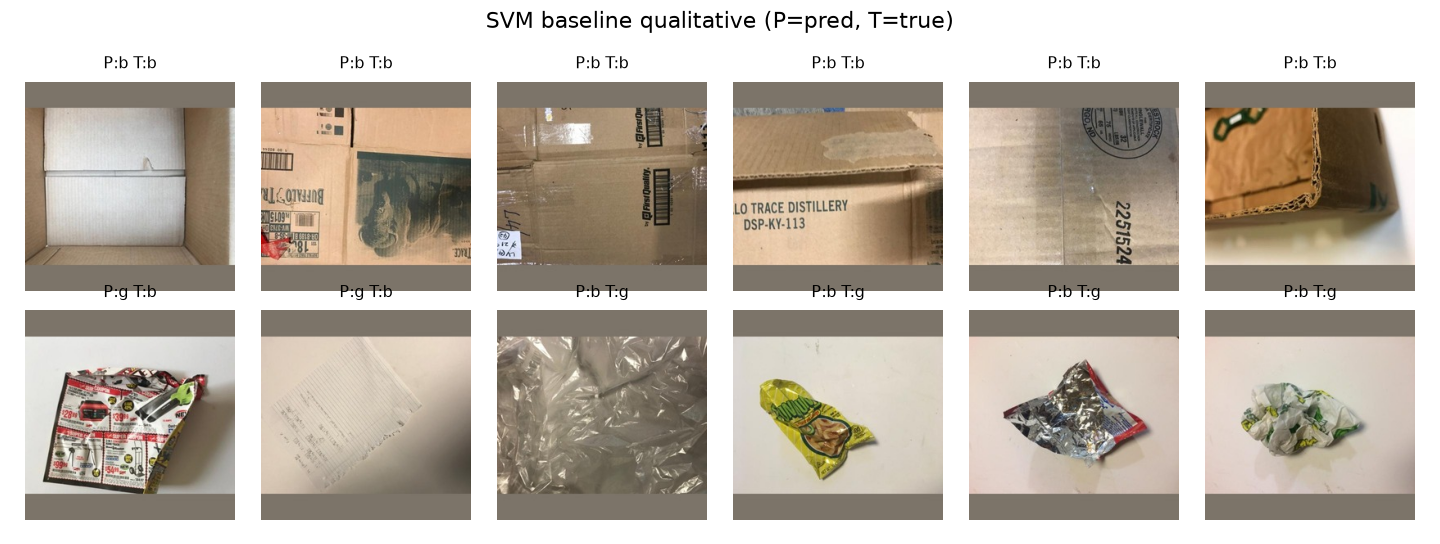
\includegraphics[height=2.7cm]{../results/svm_qualitative.png}
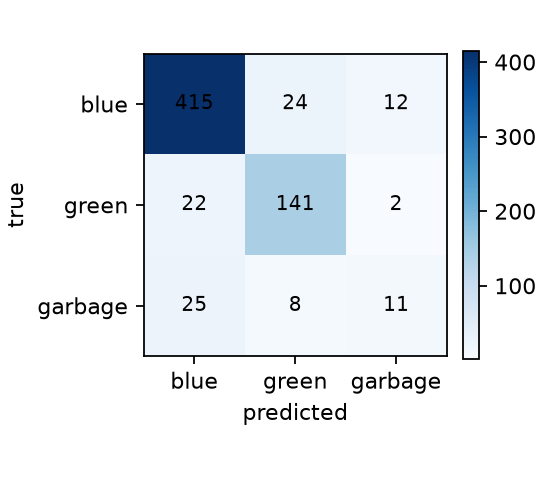
\includegraphics[height=2.7cm]{../results/svm_confusion.png}
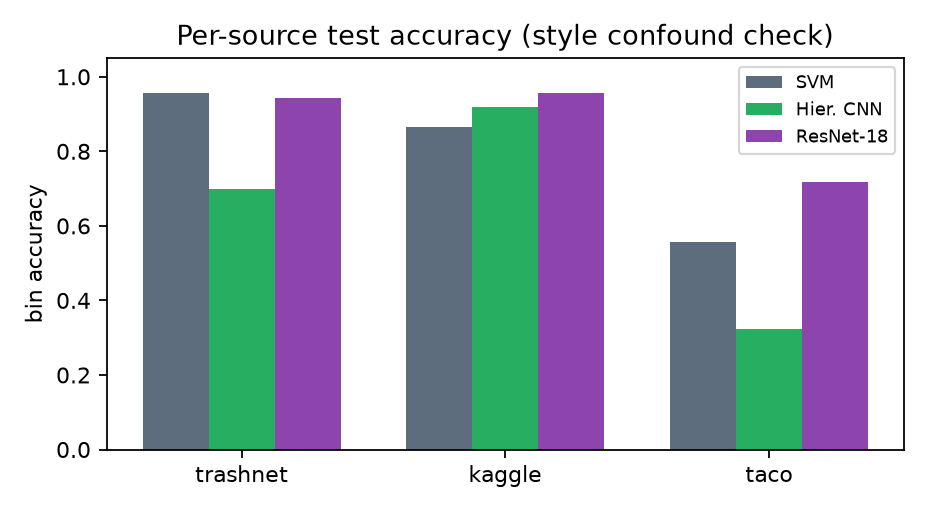
\includegraphics[height=2.7cm]{../results/per_source_accuracy.png}
\caption{SVM qualitative examples and confusion matrix (Garbage is hard); per-source accuracy shows TACO is much harder than TrashNet/Kaggle for every model.}
\label{fig:svm}
\end{figure}

\textbf{Reading the baselines.} SVM already gets 0.859 / 0.687, so a neural net cannot win just by ``being deep''. Garbage recall is only $\sim$0.25, and TACO-source accuracy falls to 0.556 (vs TrashNet 0.957). ResNet-18 is stronger (0.905 / 0.811), which makes sense with ImageNet features. Together they give a clear must-beat / must-approach target for my own CNN.

\section*{Primary Model}
\textbf{Design (mine).} My primary model is a small CNN trained from scratch. Four conv blocks ($3{\to}32{\to}64{\to}128{\to}256$; each Conv--BN--ReLU$\times2$ + MaxPool) end in GAP to 256-d with dropout 0.3. The hierarchical head is the part I care about most: material head Linear($256,7$) produces $p_{\text{mat}}$; a learnable rule matrix $R\in\mathbb{R}^{7\times3}$ makes a soft prior $p_{\text{prior}}=p_{\text{mat}}R$; a correction MLP ($256{\to}128{\to}3$) can override that prior; bin logits are $\log(p_{\text{prior}})+\mathrm{correction}$. In student language: first ask ``what is it made of?'', then ``which bin does Toronto usually want?'', then allow a small residual fix when the rule is incomplete. That is exactly the proposal insight encoded in the architecture.

I train with Adam and weighted CE (Blue dominates). Locally I only have CPU---each epoch takes several minutes, and longer overnight runs stalled when the laptop slept---so the best checkpoint I report is epoch 5. The model still has only \textbf{1.21M parameters}, about $9\times$ smaller than ResNet-18.

\begin{table}[!h]
\centering
\caption{Primary hierarchical CNN vs both baselines (cleaned test split).}
\label{tab:primary}
\scriptsize
\begin{tabular}{lrrrr}
\toprule
Model & \#params & Test bin acc. & Macro-F1 & Mat.\ acc. \\
\midrule
Hierarchical CNN (primary) & 1.21M & 0.682 & 0.557 & 0.462 \\
ResNet-18 (strong baseline) & 11.3M & 0.905 & 0.811 & 0.835 \\
HOG+HSV+SVM & --- & 0.859 & 0.687 & --- \\
\bottomrule
\end{tabular}
\end{table}

\begin{figure}[!h]
\centering
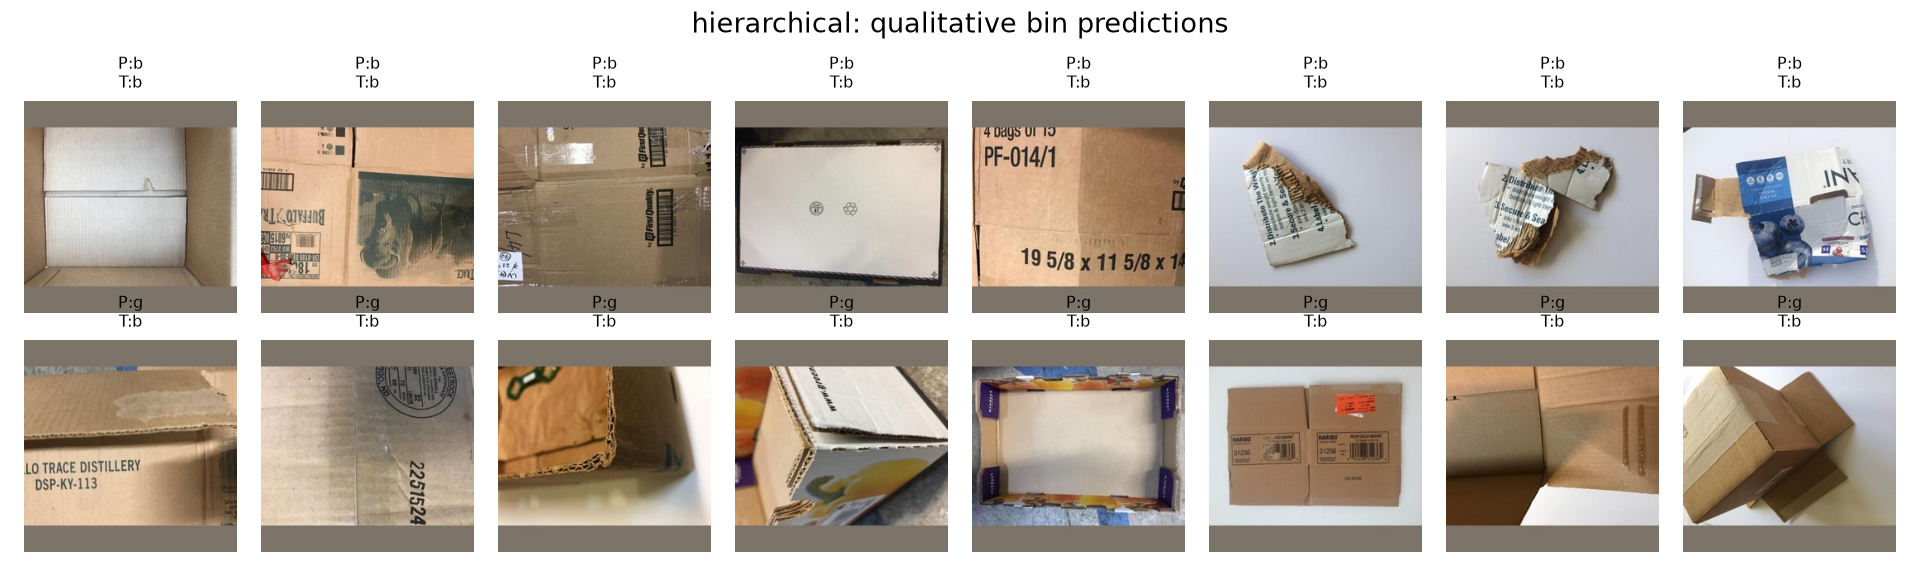
\includegraphics[height=2.75cm]{../results/hierarchical_qualitative.png}
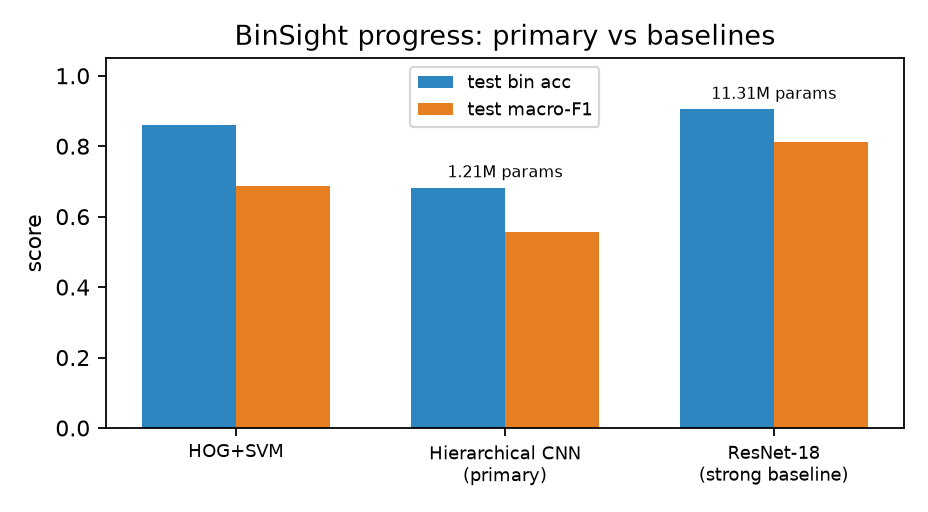
\includegraphics[height=2.75cm]{../results/model_comparison.png}
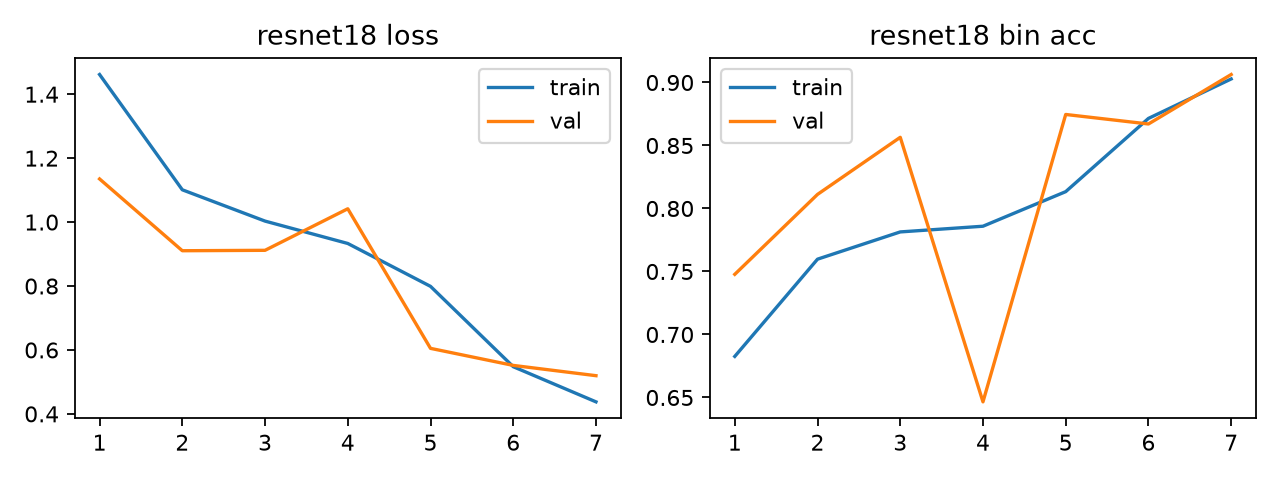
\includegraphics[height=2.75cm]{../results/resnet18_curves.png}
\caption{Hierarchical CNN qualitative predictions; quantitative comparison of all three models; ResNet-18 training curves (freeze then fine-tune).}
\label{fig:primary}
\end{figure}

\textbf{What the numbers mean to me.} Right now the ranking is ResNet-18 $>$ SVM $>$ my hierarchical CNN (0.682 / 0.557). That is a little humbling, but also useful. The from-scratch net already beats chance by a lot, and on Kaggle-source images it reaches about 0.92 bin accuracy, so it \emph{is} learning Green vs other bins. The weak spot is TACO ($\sim$0.32): messy outdoor crops are still hard after only five CPU epochs. Material accuracy (0.462) is only moderate too, which matters because the hierarchical prior depends on a decent material guess. I read this as a feasibility win more than a final accuracy win: the data pipeline works, both baselines work, and my own architecture trains and produces sensible qualitative examples. Closing the gap with longer GPU training is the natural next step, not a reason to abandon the design.

\textbf{Feasibility.} At this checkpoint I have a cleaned remapped dataset, a classical SVM baseline, a strong ResNet-18 baseline, and a personally designed hierarchical CNN with parameter count, metrics and example predictions. Completing the project on schedule looks realistic.

\newpage
\bibliographystyle{plain}
\bibliography{references}
\end{document}
